\
\section{Thermal Imaging System}

\subsection{Imaging Device}

\begin{figure}
	\centering
	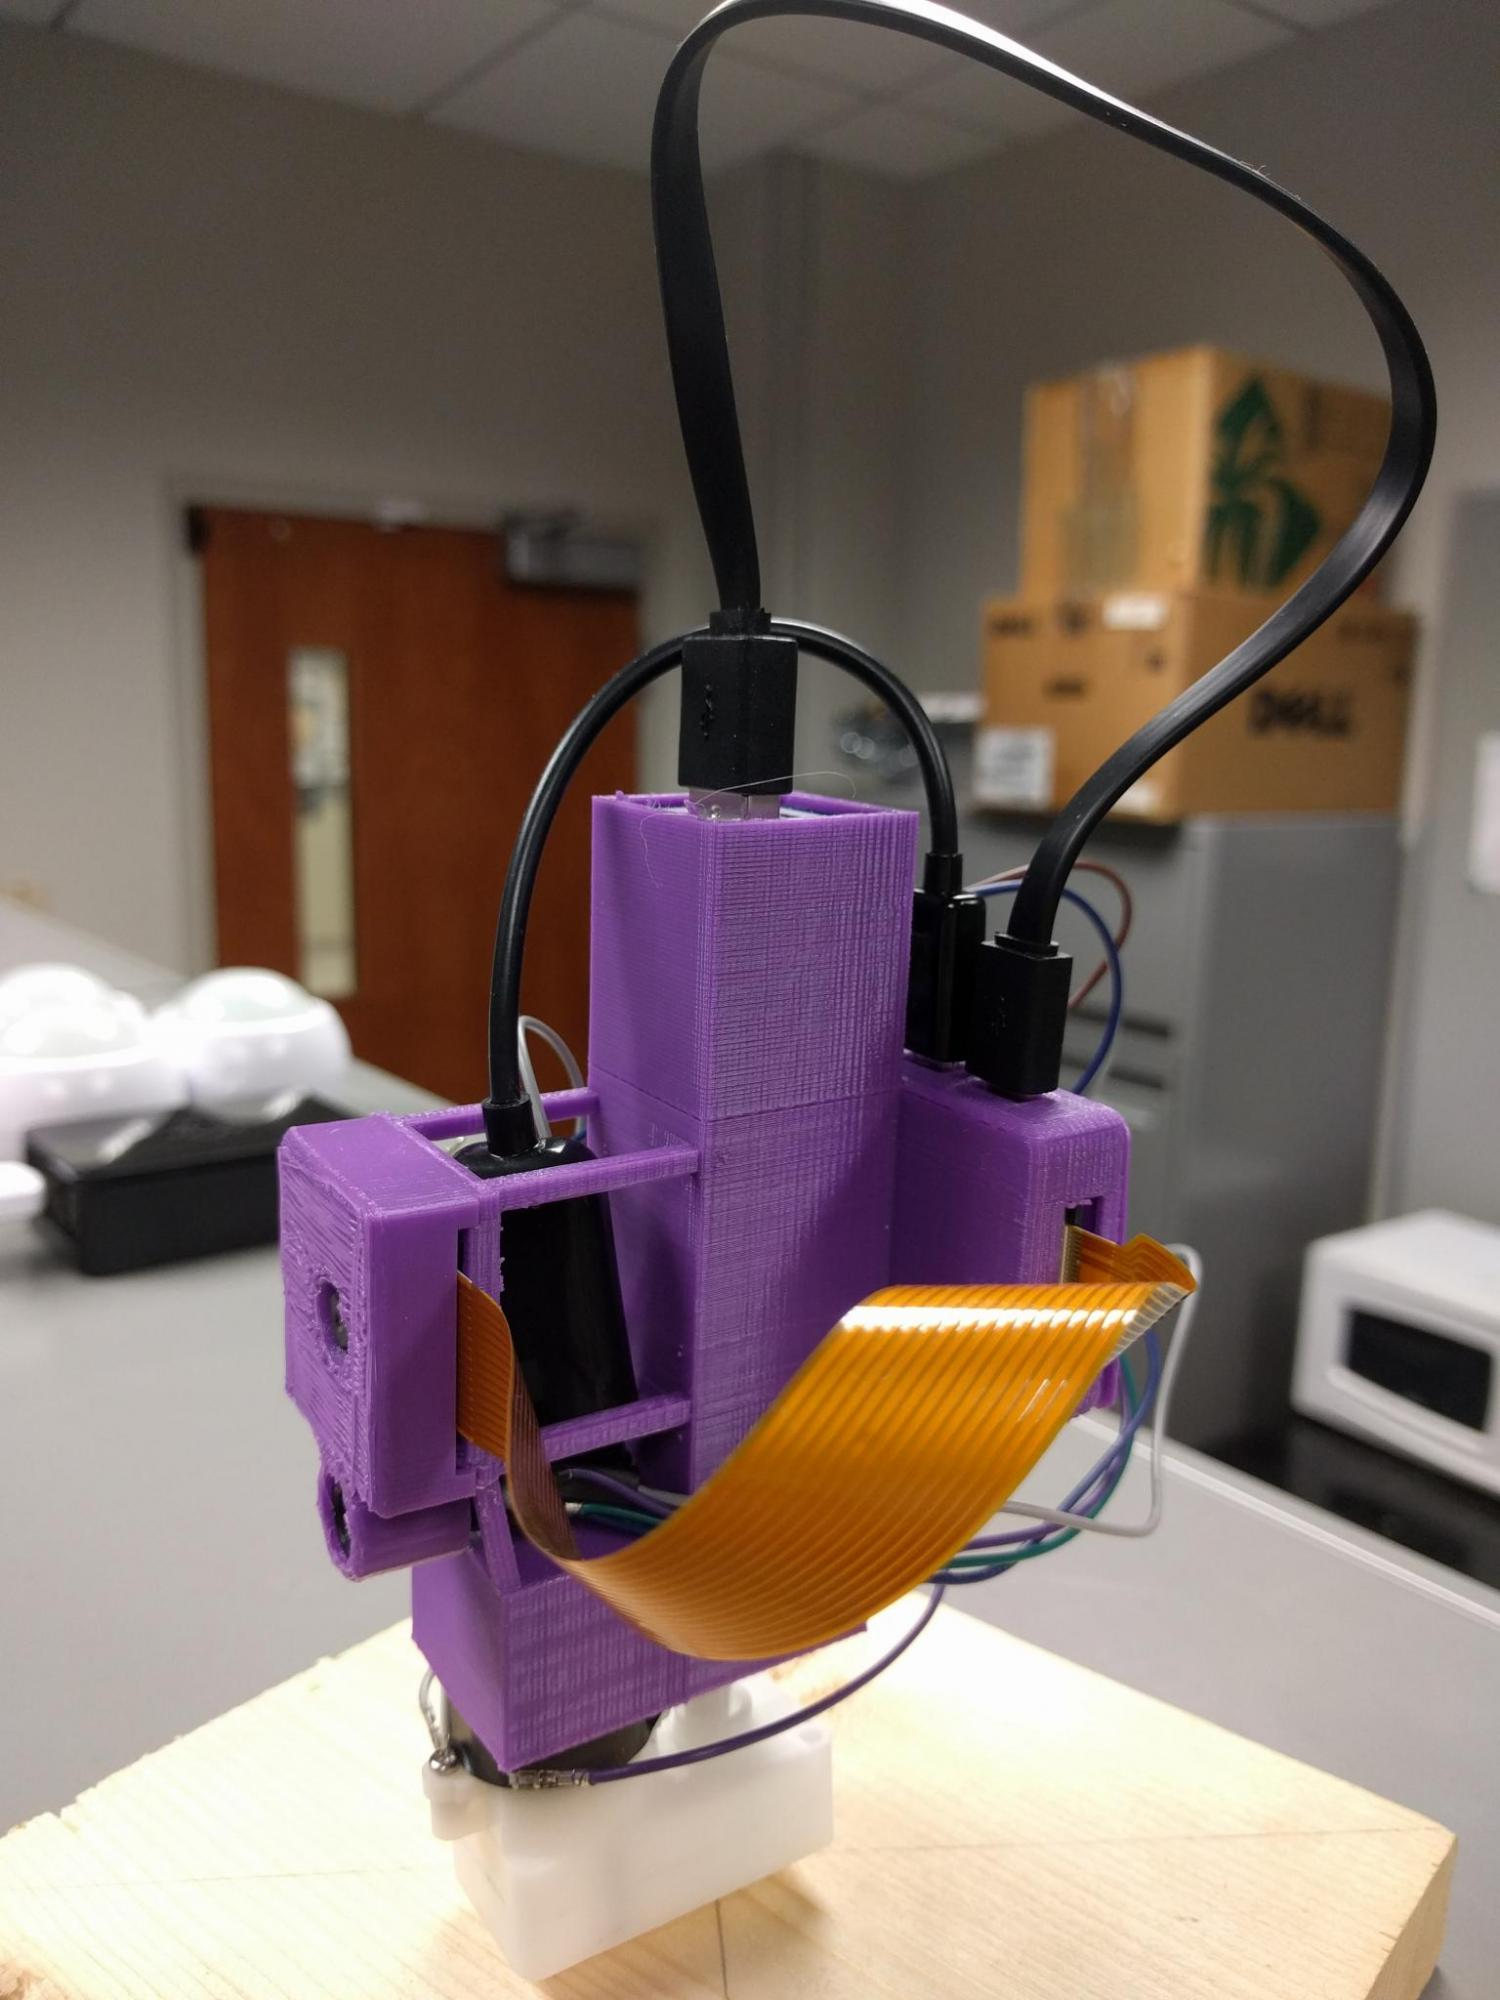
\includegraphics[height=.45\textheight,width=.45\textwidth,keepaspectratio]{../img/CameraModule.jpg}
	\caption[Imaging Device]{A prototype imaging device. The Pi Zero is on the
		right, in the rear of the device. The cameras are left, the Pi Camera 
		Module above the IR camera. The battery is in the middle of the device
		and a Wi-Fi adapter between the cameras and the battery. The motor is
		at the bottom.}
	\label{tis:imd:cam}
\end{figure}

The physical component of the thermal imaging system is a custom-created imaging
device as pictured in Figure~\ref{tis:imd:cam}. Our prototypes are built from a
Raspberry Pi Zero, a Raspberry Pi Camera Module, and a low-resolution IR camera,
powered by a $5V$ battery, rotating on a DC motor, in a 3D printed housing. This
sensor's purpose is to collect data from which to create a longitudinal thermal
map of a room and from which to detect the variations representing leakages and
other energy waste.

There are two cameras in the imaging device. The IR camera is a Melexis MLX90621
[1]. It has a low $16x4$ resolution and low power consumption of $<9mA$ when
active and $<7\mu A$ otherwise. It can detect ambient temperature between
$-40\deg C$ and $85\deg C$ and object temperatures between $-50\deg C$ and
$300\deg C$ with a resolution of $0.02\deg C$. The Raspberry Pi Camera Module [2]
is a RGB camera and collects images at $720x480$ resolution. The 3D printed 
housing holds the cameras in a consistent relative position and orientation.

The Raspberry Pi Zero controls the device. Periodically, the Pi causes the device
to rotate by steps on the motor for a number of steps sufficient to rotate at
least $360\deg$. For every step, the Pi collects a simultaneous image from each
camera. After the batch of rotations completes, the imaging device uploads the 
collected images to a server for processing.

\subsection{Image Processing}

\begin{figure*}
	\centering
	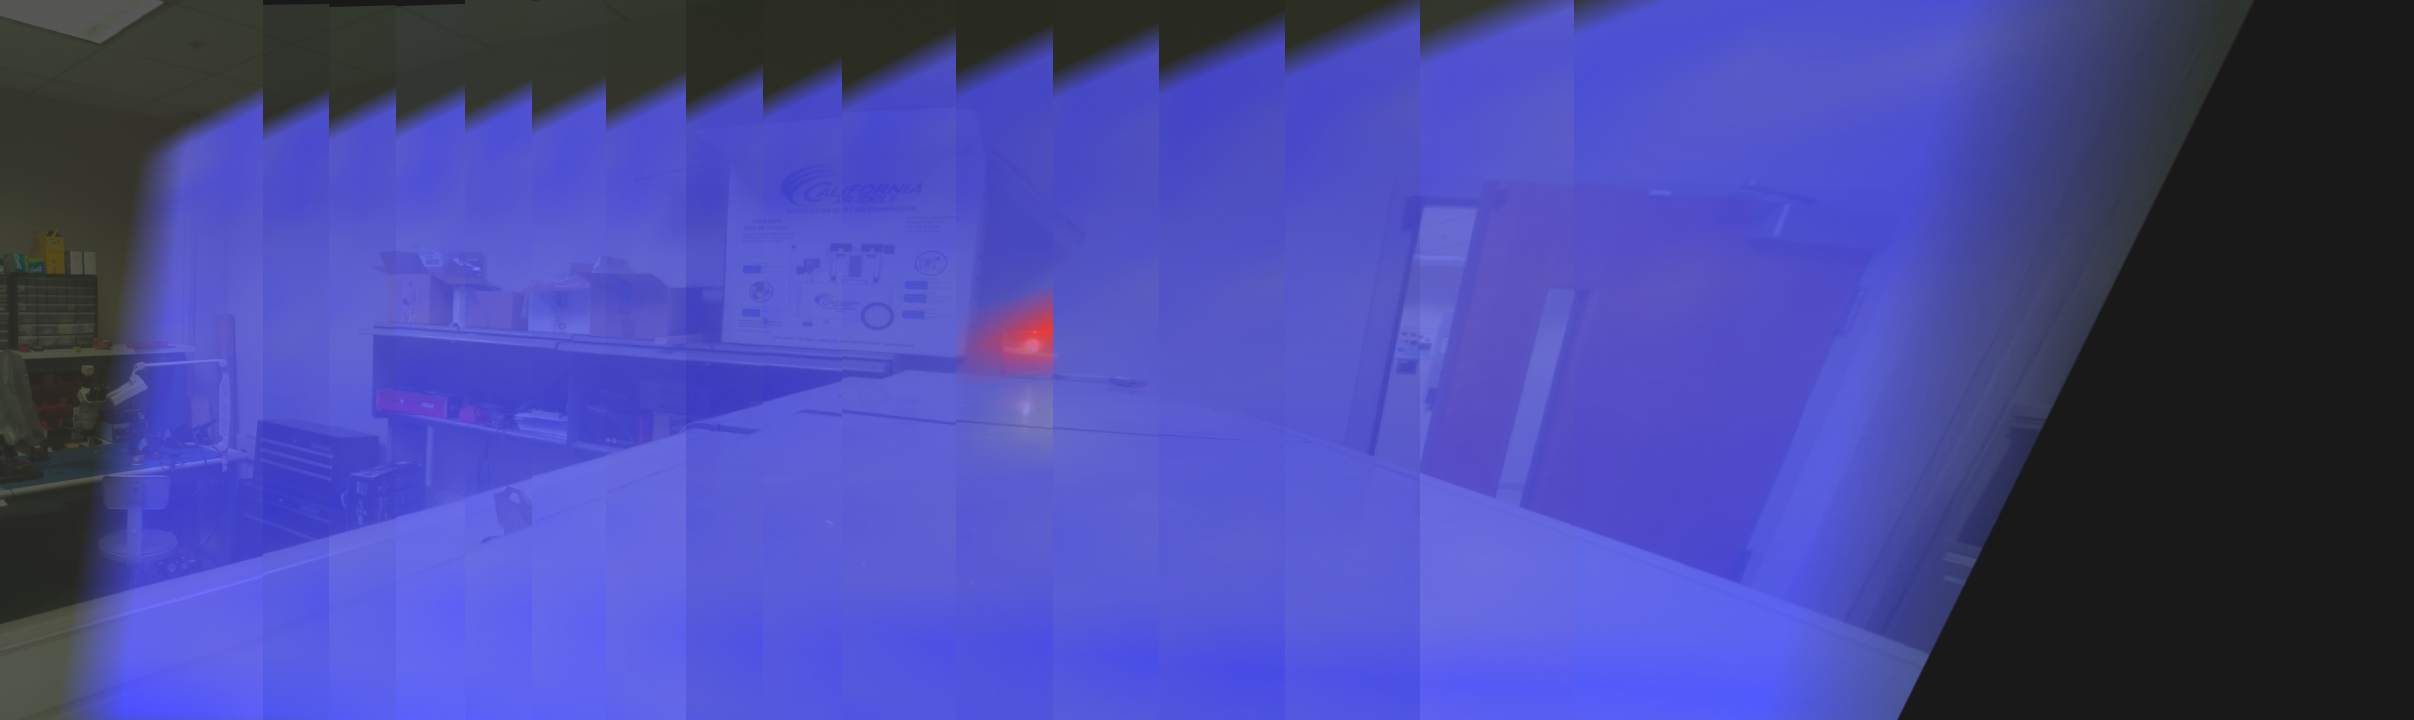
\includegraphics[height=.45\textheight,width=.75\textwidth,keepaspectratio]{../img/overlay.png}
	\caption[Stitched image]{An example stitched image detecting a candle. We 
		should get around to finding a better picture.}
	\label{tis:imp:ex}
\end{figure*}

On the image processing server, we use the RGB and IR image sets to generate a 
unified thermal map of the room. The first image processing step uses OpenCV [3]
to generate a panorama from the RGB images and record the homography matrices
used for those image transformations. This process allows us to avoid the need
for a heavier, more expensive stepper motor, because those homography matrices
encode the relationships between sequential images. The second step uses those 
matrices to produce an IR panorama of the room. The 3D printed housing of the
imaging device maintains a fixed relationship between the positions and
perspectives of the two cameras in each prototype. We calculate the mapping
between the cameras once and, at processing time, use this transformation in
addition to the homographies calculated in the RGB stitching process. Thus, we
map each IR image on to its corresponding RGB image, then stitch those
transformed IR images to create an IR panorama of the room.

% Stitch images
% Overlay IR
% Don't need heavier, more expensive, more complicated motor

[1] https://www.melexis.com/en/product/MLX90621/Far-Infrared-Sensor-Array-High-Speed-Low-Noise
[2] https://www.raspberrypi.org/products/camera-module-v2/
[3] @article{opencv_library,
	author = {Bradski, G.},
	citeulike-article-id = {2236121},
	journal = {Dr. Dobb's Journal of Software Tools},
	keywords = {bibtex-import},
	posted-at = {2008-01-15 19:21:54},
	priority = {4},
	title = ,
	year = {2000}
}